\subsection*{Daglig helbredstilstand}
Førend en træning påbegyndes skal brugerens daglige helbredstilstand angives. Dette er for at sikre, at træningen tilpasses den individuelle bruger samt imødekomme dag til dag variationer. Af \autoref{fig:helbredstilstand} fremgår aktivitetsdiagrammet for angivelse af den daglige helbredstilstand. 

\begin{figure} [H]
\centering
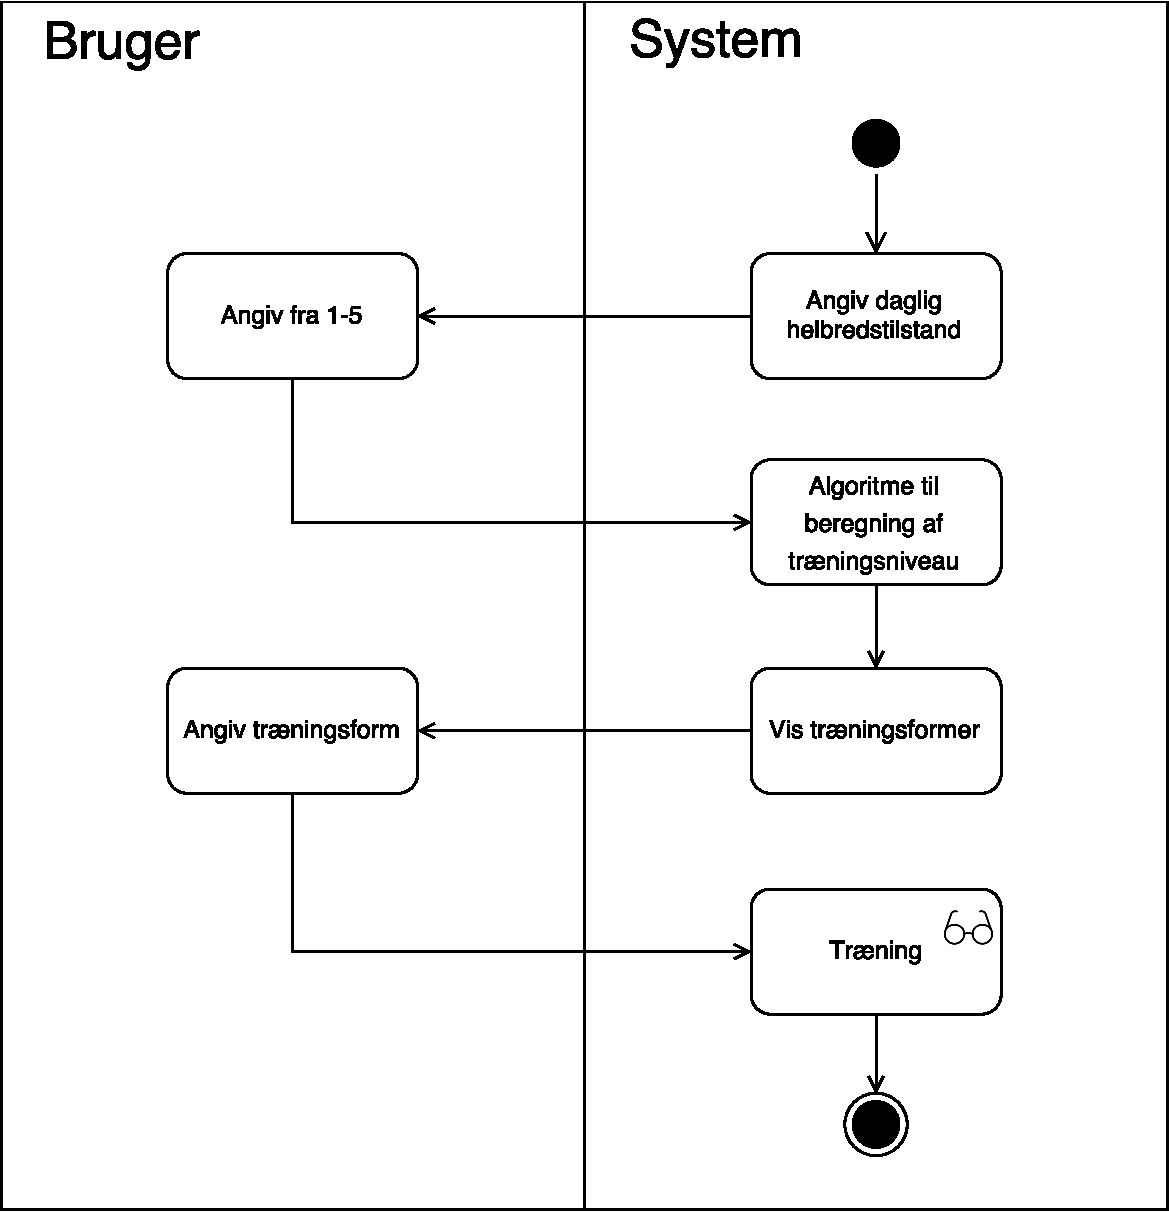
\includegraphics[width=0.9\textwidth]{figures/aktivitetsdiagram/Helbredstilstand}
\caption{Aktivitetsdiagram for daglig helbredstilstand. Træning er yderligere beskrevet af \autoref{fig:traening}.}
\label{fig:helbredstilstand}
\end{figure}

\noindent
Den daglige helbredtilstand angives ved hjælp af en skala fra 1, svarende til en dårlig helbredstilstand, til 5, svarende til en god helbredstilstand. Ud fra den daglige helbredstilstand, kategoriseringen af KOL samt evaluering fra førhenværende træning, passende til den angivede helbredstilstand, vælges et træningsniveau passende til brugerens nuværende helbred. Dertil foreslås brugeren forskellige træningsformer, herunder konditions-, styrketræning samt vejrtrækningsøvelser. Den ønskede træningsform vælges, hvortil træningen kan udføres. Træningen er yderligere beskrevet af \autoref{fig:traening}. 


*** Beslutningstræ! ***